As is shown in Sec.~\ref{sec:beamDyn}, the longitudinal force on a charged particle in a particle accelerator is defined as 

\begin{equation}
F_{\parallel} = qE_{z}.
\label{eqn:longForce}
\end{equation}

Often it is useful to take into account the change in energy in a particle, thus we can transform Eqn.~\ref{eqn:longForce} to

\begin{equation}
\frac{dE}{dz} = v\frac{dp}{dz} = \frac{dp}{dt} = eE_{z}
\end{equation}

where $dE$ is the infinitessimal energy change of the particle, $dp$ the infintessimal momentum change. Here we assume relativistic dynamics where 

\begin{equation}
E^{2} = E_{0}^{2} + p^{2}c^{2}
\end{equation}

where $E_{0}$ is the particles rest energy and $c$ the speed of light. The change in kinetic energy $W$ from the particle traversing a path $z$ is given by

\begin{equation}
\Delta W = \int dE = \int \mathbf{dz}.\mathbf{\hat{z}} E_{z} e = eV
\end{equation}

where $V$ is the potential seen by the charged particle. Typically the electric field of an RF cavity is an oscillating field with an angular frequency $\omega_{rf}$, giving an electric field at some time $t$

\begin{equation}
E_{z} = E_{0} cos \left( \omega_{rf} t \right)
\end{equation}

where $E_{0}$ is the field magnitude. If we consider a particle beginning its traversal of the electric field (located between $z=-L_{cav}/2$ and $z=L_{cav}/2$) at $t=0$ (such that $z=vt$) we find that

\begin{equation}
\Delta W = \frac{e}{L_{cav}} \int^{\frac{L_{cav}}{2}}_{\frac{-L_{cav}}{2}} dz E_{z}\left( z \right) cos \left( \omega_{rf} \frac{z}{v} \right).
\end{equation}

Another way to represent the change in kinetic energy is by the use of a factor known as the time transit factor, commonly represented by $T$. To illustrate it's used consider the general case of energy change $\Delta W$, and use complex notation we have

\begin{equation}
\Delta E = \frac{e}{L_{cav}} \Re{}e \left[ \int^{\frac{L_{cav}}{2}}_{\frac{-L_{cav}}{2}} dz E_{z}\left( z \right)e^{j \omega_{rf} t}.\right]
\end{equation}

If we have a particle with a phase $\Phi_{p}$ relative to the RF phase ($\omega_{rf}t = \omega_{rf}z/v - \Phi_{p}$) leading the equation to become

\begin{equation}
\Delta E = e \Re{}e \left[ e^{-j \Phi_{p}}\int^{\frac{L_{cav}}{2}}_{\frac{-L_{cav}}{2}} dz E_{z}\left( z \right) e^{j \omega_{rf} \frac{z}{v}}.\right]
\end{equation}

\begin{equation}
\Delta E = e \Re{}e \left[ e^{-j \Phi_{p}} e^{-j \Phi_{i}} \left| \int^{\frac{L_{cav}}{2}}_{\frac{-L_{cav}}{2}} dz E_{z}\left( z \right) e^{j \omega_{rf} \frac{z}{v}}.\right| \right]
\end{equation}

where $\Phi_{i}$ is the phase of the RF. If we introduce $\phi = \Phi_{p} - \Phi_{i}$ as the phase of the particle relative to the RF this becomes

\begin{equation}
\Delta E = e  \left| \int^{\frac{L_{cav}}{2}}_{\frac{-L_{cav}}{2}} dz E_{z}\left( z \right) e^{j \omega_{rf} \frac{z}{v}}.\right| cos \phi.
\end{equation}

The time transit factor $T$ is now defined as the energy gain of a transitting particle over the maximum energy gain of a transitting particle (i.e. a particle with a velocity $v \rightarrow \infty $), such that 

\begin{equation}
T =    \frac{\left| \int^{\frac{L_{cav}}{2}}_{\frac{-L_{cav}}{2}} dz E_{z}\left( z \right) e^{j \omega_{rf} \frac{z}{v}}.\right|}{  \left| \int^{\frac{L_{cav}}{2}}_{\frac{-L_{cav}}{2}} dz E_{z}\left( z \right) \right|}.
\end{equation}

\section{Phase Stability}

A consequence of the factor $\phi$, dispersion in a circular machine and multiple particle energies in a bunch (see \cite{Leduff:LongDyn} for more details) is that for a bunch of particles interacting with an RF system there a stable phase of the particle relevant to RF phase dependent on whether it is above transition or below transition. Below transition corresponds to the situation where an increase in the energy of a particle translates into a reduction in time taken to circle the accelerator, due to the increased velocity. Above transition corresponds to the situation where an increase in energy corresponds to an increase in the time taken to circle the accelerator due to the marginal increase in velocity (due to $v \approx c$) not compensating for the increased distance travelled by the particle. Transition is the point in which these two effects cancel.

This means that the value of $\phi$ which leads to longitudinal focusing is different above and below transition energy. It can be shown that this is $\phi = \phi_{s}$ below transition and $\phi = \pi - \phi_{s}$ above transition, where $\phi_{s}$ is the synchronous phase for the desired motion ($\phi_{s} = 0$ for no acceleration, $\phi_{s} < 0$ for deceleration and $\phi_{s} > 0$ for acceleration). This is illustrated in Fig.~\ref{fig:longPhase}, where position $P_{1}$ indicates the phase position below transition and $P_{2}$ above transition.

\begin{figure}
\begin{center}
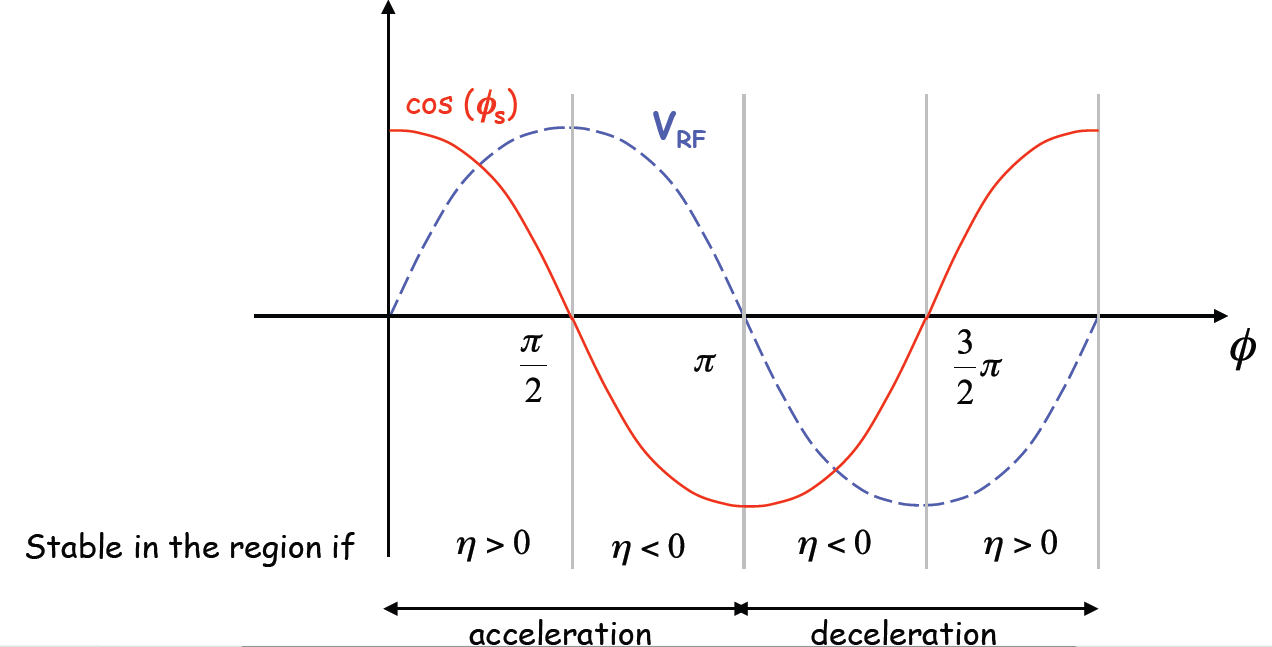
\includegraphics[width=0.75\textwidth]{appendices/figures/longStab.png}
\end{center}
\caption{The focusing synchronous phase positions for particle below ($P_{1}$) and above ($P_{2}$) transition. The synchronous phase is chosen for a given particle energy and desired behaviour, and an off-momentum particle will be longitudinally focused to the synchronous phase by the RF system if the correct phase is chosen. This occurs due to balance of increased velocity with an increased size of orbit as a particle is accelerated by the RF electric field.}
\label{fig:longPhase}
\end{figure}

\section{RF Acceptance and Longitudinal Emittance}

To examine longitudinal motion of bunches it often easier to work with the conserved longitudinal quantities as with the transverse plane. These two variables turn out to be $\phi$, the phase of the particle and a variable $W$, related to the momentum of the particle. These are equivalent to the displacement $x$ and transverse momentum $p_{x}$ in transverse motion ($\phi$ effectively being the displacement of the off-momentum particle normalised by the RF wavelength). The product of these is a preserved quantity, known as the seperatrix.

One interesting side effect of the stable phase condition is that the largest seperatrix exists when $\phi_{s}= 0$ or $\pm \pi$, i.e. when no acceleration of the particles occurs. It can be shown that as stronger and stronger acceleration (the energy gain per turn increases) is applied, the seperatrix decreases in area, as shown in Fig.~\ref{fig:longSynFreq}, reaching it's smallest value at $\phi_{s} = \pi / 2$.

\begin{figure}
\begin{center}
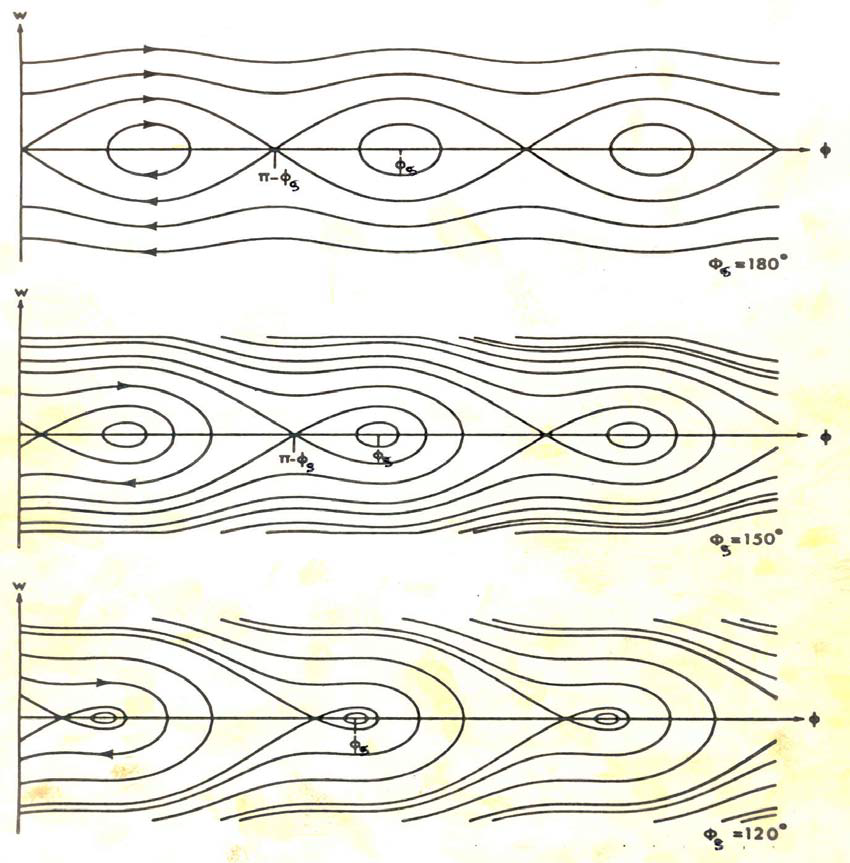
\includegraphics[width=0.75\textwidth]{appendices/figures/longPhaseDiag.png}
\end{center}
\caption{The stable longitudinal phase area (seperatrix) for different synchronous phase values. Note that the seperatrix decreases in volume as $\phi_{s} \rightarrow \pi / 2$.}
\label{fig:longSynFreq}
\end{figure}